\chapter{Az S-gráf keretrendszer}
Az S-gráf keretrendszer volt az első publikált gráf elméleten alapuló módszer szakaszos gyártórendszerek ütemezési problémáinak megoldására. \cite{Sanmarti2002}
A keretrendszer egy irányított gráf modellből, az S-gráfból és a hozzá tartozó algoritmusokból áll. \cite{SANMARTI1998S847}
Az S-gráf egy speciális irányított gráf, amely nem csupán a probléma vizualizációjára képes, hanem egy matematikai modell is.
A keretrendszerben a recepteket, valamint a félkész-, illetve a teljes ütemterveket is az S-gráf reprezentálja.
Ezekben a gráfokban a termékeket, illetve a feladatokat a pontok jelölik, amelyeket csomópontoknak nevezünk.
Ezenkívül, ha két feladat között összeköttetés van, ezt a gráfon a két feladatot reprezentáló csomópontok közötti nyíl jelöli.
Az ütemezési információ nélküli S-gráfot recept gráfnak (\textbf{recipe graph)} nevezzük, melyre egy példa a \ref{recipeGraph} ábrán látható.
\begin{figure}[H]
\begin{center}
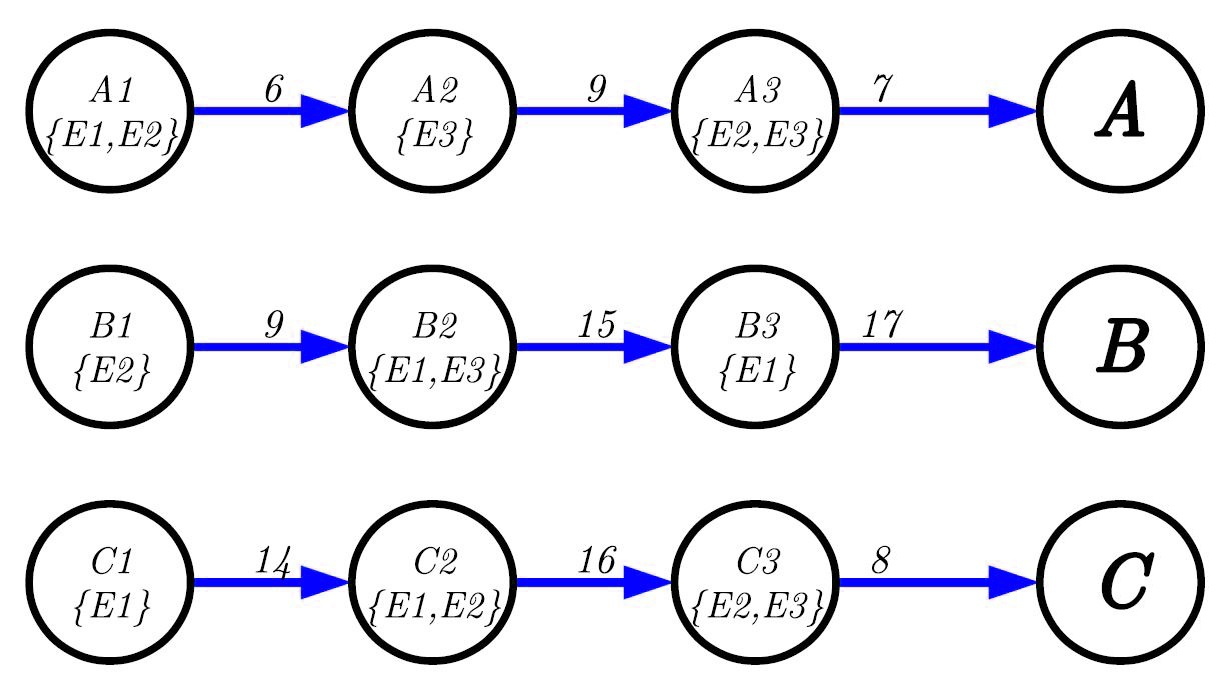
\includegraphics[scale=0.35]{recipeGraph}
\caption{A recept gráf szemléltetése}
\label{recipeGraph}
\end{center}
\end{figure}
Az ábrán látható jobb oldali három csomópont (A,B,C) jelöli a termékeket, a többi csomópont pedig a részfeladatokat, amelyeket el kell végezni a termékek előállítása érdekében.
A recept gráf nyilai reprezentálják egyrészt két részfeladat közötti függőséget, abban ez esetben például, ha ez egyik részfeladat állítja elő a másik részfeladathoz szükséges bemeneti részterméket, másrészt a részfeladatok és a késztermékek közötti függőséget.
A recept gráf minden részfeladathoz tartozó csomópontjához tartozik egy halmaz, amely azon berendezések nevét tartalmazza, amelyek képesek adott részfeladat megoldására.
A nyilakon található súlyok pedig a részfeladat megoldásához szükséges gyártási időt reprezentálják, abban az esetben, ha egy részfeladatot több berendezés is el tud végezni, a nyíl súlya a berendezésekhez tartozó gyártási idők közül a legkisebb lesz.

Az S-gráf keretrendszerben található algoritmusok az előzőekben bemutatott recept gráfot egészítik ki ütemezési nyilakkal, amelyek az algoritmus által meghozott ütemezési döntéseket reprezentálják.
Az ily módon előállított gráfot, függetlenül attól, hogy van-e még meghozatlan ütemezési döntés, vagy pedig a teljes ütemezés megtörtént, ütemezési gráfnak (\textbf{schedule graph}) nevezzük.
A \ref{recipeGraph} pontban látható recept gráf alapján előállított ütemezési gráf a \ref{scheduleGraph} ábrán látható.
\begin{figure}[H]
\begin{center}
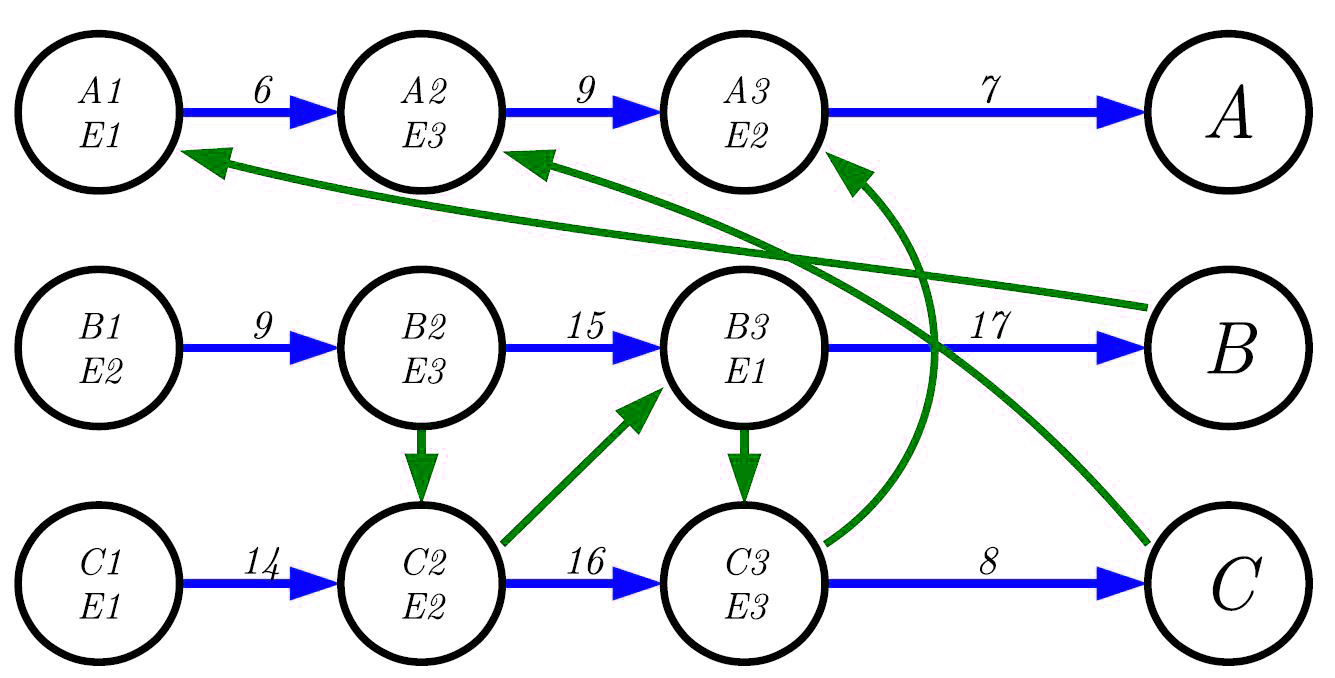
\includegraphics[scale=0.3]{scheduleGraph}
\caption{Az ütemezési gráf szemléltetése}
\label{scheduleGraph}
\end{center}
\end{figure}
Az ábrán látható gráfon már minden ütemezési döntés lezajlott, a zöld nyilak jelölik az ütemező algoritmus által behúzott ütemezési nyilakat.
A részfeladatokat reprezentáló csomópontokon immáron a lehetséges berendezések halmaza helyett egy konkrét berendezés jelölése található, amely az adott részfeladat elvégzésére hivatott az adott ütemterv szerint.
Az ütemezési nyilak súlya alapértelmezetten $0$, ha az adott problémában nem számolunk például részfeladatok közötti szállítási-, átállási-, illetve tisztítási időkkel.
Az adott berendezéshez rendelt részfeladatok sorrendje könnyen leolvasható az ütemezési gráfról, erre egy példa a \ref{unitSequence} ábrán látható.
\begin{figure}[H]
\begin{center}
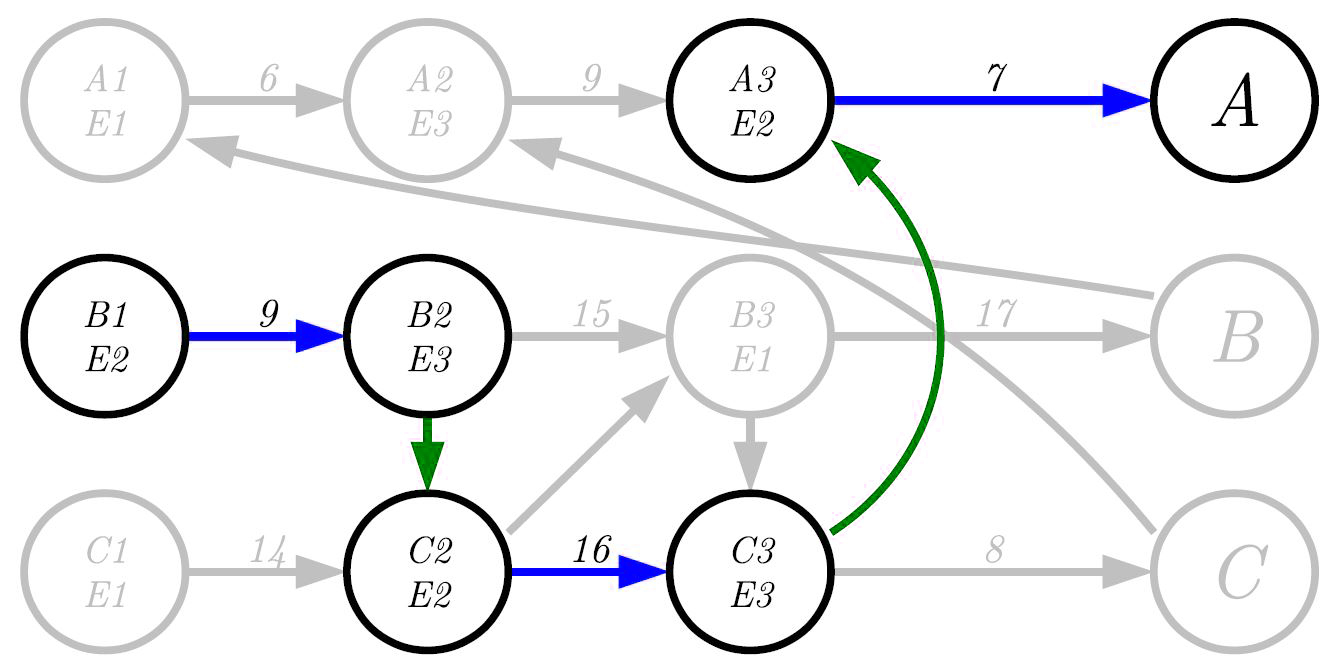
\includegraphics[scale=0.3]{unitSequence}
\caption{Az E2 berendezéshez rendelt részfeladatok sorrendje}
\label{unitSequence}
\end{center}
\end{figure}
Az ábra alapján leolvasható, hogy az E2 berendezés először a B1 részfeladatot végzi el, majd a C2, azután pedig az A3 fog következni.
Ahhoz azonban, hogy például a C2 részfeladatot E2 berendezés el tudja végezni, nem elegendő az, hogy B1 befejeződjön, elengedhetetlen az is, hogy minden részfeladat amitől C2 függ (nevezetesen C1) szintén véget érjen.

Az S-gráf keretrendszerben történő ütemezésre egy bővebb példa a makespan minimalizáló \footnote{A makespan minimalizáló algoritmus segítségével adott receptgráffal reprezentált termékek gyártási ideje minimalizálható. Az algoritmus fontos szerepet játszik a \ref{SgraphProfitMax}. alfejezetben tárgyalt profit (throughput) maximalizáló algoritmusban is.} algoritmuson keresztül szemléltetve megtalálható a CD melléklet \fileName{Algoritmusok} mappájában \fileName{DO\_Sgraph\_Makespan\_Minimization.odg} néven. 
\section{Profit maximalizálás az S-gráf keretrendszerrel} \label{SgraphProfitMax}
Az S-gráf keretrendszer eredetileg makespan minimalizációs célokra lett megalkotva, azonban később kibővítésre került egy throughput maximalizáló algoritmussal, amely segítségével immáron profit maximalizálásra is képes.
Az throughput maximalizáló algoritmus alapötletét Majozi és Friedler \cite{doi:10.1021ie0604472}, valamint Holczinger \cite{HOLCZINGER2007649} fektették le, melynek lényege, hogy a termékek lehetséges batch darabszámai alapján különböző konfigurációk kerülnek létrehozásra\footnote{A és B termékek esetén egy lehetséges konfiguráció például, ha A termékből 1 darab, B-ből 2 darab batch-et gyártunk.}, melyek között branch \& bound algoritmus segítségével eredményül kapható a legnagyobb profitot eredményező konfiguráció, ha létezik megvalósítható (feasible) megoldás a problémára.

A throughput maximalizáló algoritmus működésének egy példán keresztül történő szemléltetésére készült folyamatábra a CD melléklet \fileName{Algoritmusok} mappájában található \fileName{DO\_Sgraph\_Throughput\_Maximization.odp} néven.
Kezdetben a konfigurációk halmaza tartalmazza az összes lehetséges konfigurációt az adott termékekre, majd minden iteráció során kiválasztásra kerül egy konfiguráció, amelynek teszteljük feasible-itását, azaz hogy a rendelkezésre álló időhorizont alatt megvalósítható-e adott konfiguráció legyártása.
Ennek tesztelése a korábban már említett makespan minimalizáló algoritmus felhasználásával a legegyszerűbb.
A makespan minimalizáló algoritmusnak átadásra kerül adott konfiguráció recept gráfja, majd az eredményül kapott idő érték összehasonlításra kerül a rendelkezésre álló időhorizonttal, ha a kapott érték nagyobb annál, az adott konfiguráció nem valósítható meg (infeasible). 
Ha az adott konfiguráció megvalósítható a rendelkezésre álló időhorizont alatt, kiszámításra kerül az adott konfiguráció által nyújtott profit, ha ez nagyobb az eddigi legjobb értéknél, frissíteni kell a legjobb értéket adott konfiguráció revenue értékével.
Kezdetben a tengelyek menti konfigurációk kerülnek tesztelésre mind addig, még az összes tengelyen el nem jutunk az első megvalósíthatatlan (infeasible) konfigurációig.
Ezzel előáll egy tér, amely tartalmazza az optimális megoldást, amelyet már csak meg kell találni, mivel azonban a konfigurációk tesztelése erőforrás igényes feladat, ezért a konfigurációk kiválasztásának sorrendje nem mindegy, többféle stratégia létezik az algoritmus gyorsítására. \cite{phd_Hegyhati}
Az egyik ilyen stratégia az úgynevezett revenue line behúzása, mely segítségével szerencsés esetben akár töredékére csökkenthető a tesztelendő konfigurációk száma.
A revenue line segítségével lényegében eltávolításra kerülnek azok a konfigurációk, melyek profitja nem éri el az aktuális legjobb profit értéket, azaz a behúzott vonal alatt vannak.
A revenue line szemléltetésére a \ref{revLine} ábra hivatott, mely a már fent említett  \fileName{DO\_Sgraph\_Throughput\_Maximization.odp} fájl részlete.
 \begin{figure}[H]
\begin{center}
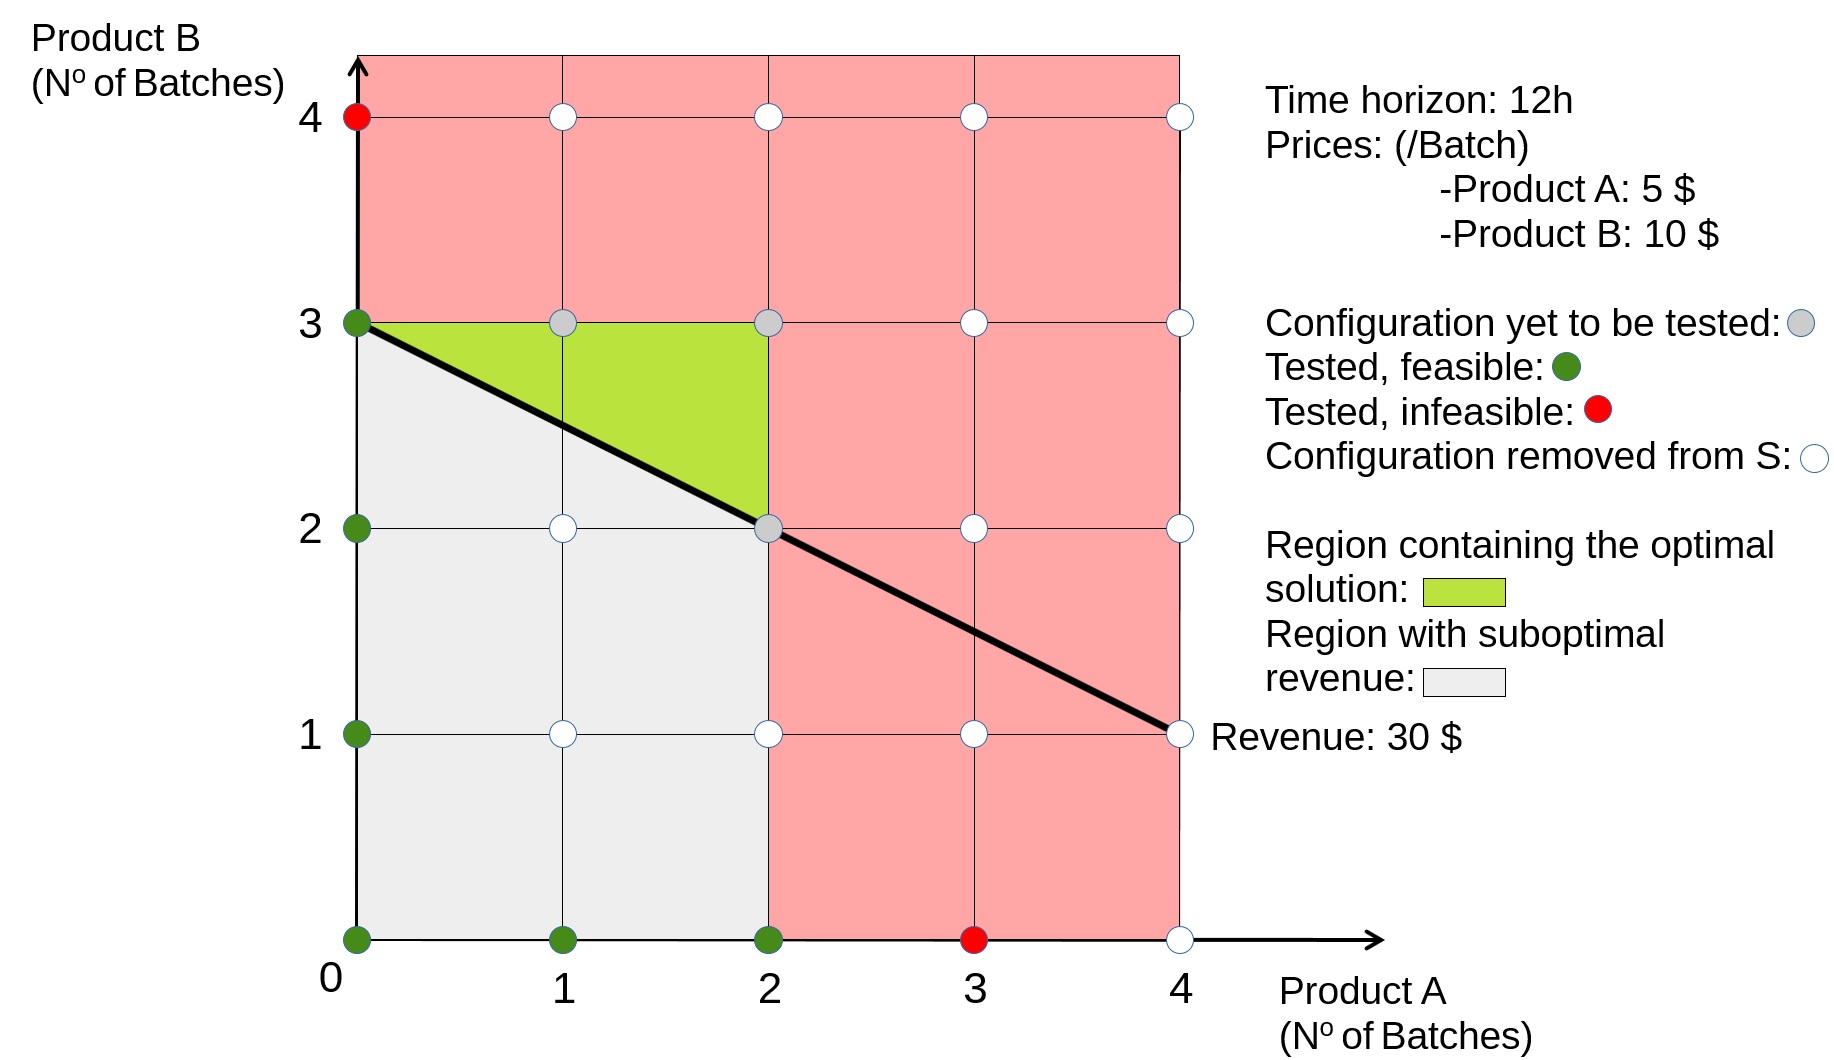
\includegraphics[scale=0.3]{revLine}
\caption{A revenue line szemléltetése}
\label{revLine}
\end{center}
\end{figure}
Jól látható, hogy jelen esetben a revenue line behúzása felére csökkentette az ellenőrizendő konfigurációk számát, gyorsítva ezzel az algoritmus lefutását.
Az algoritmus akkor ér véget, ha a konfigurációk halmaza kiürül, ebben az esetben ha egyetlen egy megvalósítható megoldás sem található, a probléma megoldása lehetetlen az adott időhorizont alatt.
Ha található feasible megoldás, az algoritmus az optimális konfigurációt adja eredményül, megkapva ezzel a maximális profit értékét, valamint annak előállításához szükséges ütemtervet.